\documentclass[12pt, twoside]{article}
\input{../preamble}

%\setlength{\headheight}{1in}
\fancyhead[LO]{La Scuola d'Italia / Dr.\ Huson / IB Math: Practice \\* 13 March 2026}
\fancyhead[RO]{\fbox{\begin{minipage}{6cm}\footnotesize First \& Last name:\\[0.5cm]\end{minipage}}}
\fancyfoot[C]{\thepage}

\begin{document}
\subsubsection*{11.7 Homework: Calculus Review}

\begin{center}\textbf{--- Section A: No Calculator ---}\end{center}

\begin{enumerate}[itemsep=0.15cm]

%--- Problem 1: Chain rule g(x) = e^(x^2+1), find g'(-1) [4 marks] ---
%    Source: AA SL 2022 Nov P1, Q2 (no calc)
\item[1.] [Maximum mark: 4]

The function $g$ is defined by $g(x) = \mathrm{e}^{x^{2}+1}$, where $x \in \mathbb{R}$.

Find $g'(-1)$.

\begin{tikzpicture}
  \draw (-0.6,0) rectangle (11,14);
  \foreach \y in {1,2,...,13} \draw[dotted] (0,\y)--(10.5,\y);
\end{tikzpicture}

\fancyhead[RO]{} % name box only on first page
\newpage

%--- Problem 2: Definite integration (3√x - 5)/√x [5 marks] ---
%    Source: AA SL 2022 May P1 TZ1, Q2 (no calc)
\item[2.] [Maximum mark: 5]

\begin{enumerate}[itemsep=0.1cm]
  \item The expression $\dfrac{3\sqrt{x}-5}{\sqrt{x}}$ can be written as $3 - 5x^{p}$.
        Write down the value of $p$. \hfill [1]
  \item Hence, find the value of
        $\displaystyle\int_{1}^{9}\!\left(\frac{3\sqrt{x}-5}{\sqrt{x}}\right)\mathrm{d}x$. \hfill [4]
\end{enumerate}

\begin{tikzpicture}
  \draw (-0.6,0) rectangle (11,13);
  \foreach \y in {1,2,...,12} \draw[dotted] (0,\y)--(10.5,\y);
\end{tikzpicture}

\newpage

%--- Problem 3: Tangent + product rule y = (2x-1)e^(kx) [5 marks] ---
%    Source: AA SL 2022 May P1 TZ1, Q5 (no calc)
\item[3.] [Maximum mark: 5]

Consider the curve with equation $y = (2x-1)\mathrm{e}^{kx}$, where
$x \in \mathbb{R}$ and $k \in \mathbb{Q}$.

The tangent to the curve at the point where $x = 1$ is parallel to the line
$y = 5\mathrm{e}^{k}x$.

Find the value of $k$.

\begin{tikzpicture}
  \draw (-0.6,0) rectangle (11,13);
  \foreach \y in {1,2,...,12} \draw[dotted] (0,\y)--(10.5,\y);
\end{tikzpicture}

\newpage

%--- Problem 4: Circle sector, arc length + area [6 marks] ---
%    Source: based on AA SL 2021 May P1 TZ2, Q1 (no calc); modified values
\item[4.] [Maximum mark: 6]

The following diagram shows a circle with centre O and radius $r$.

\begin{center}
\textbf{diagram not to scale}
\vspace{-0.2cm}

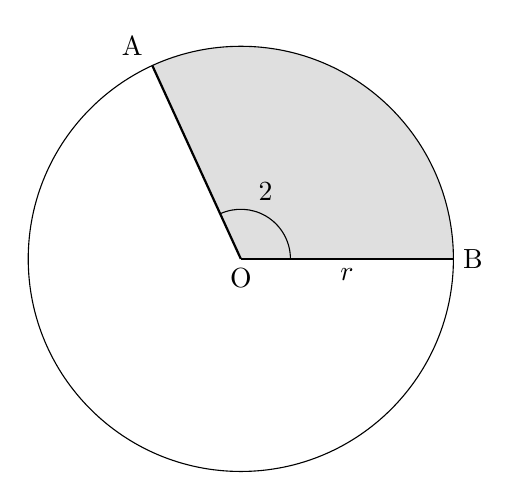
\begin{tikzpicture}[scale=0.9]
  \coordinate (O) at (0,0);
  \coordinate (B) at (3,0);
  \coordinate (A) at ({3*cos(114.6)},{3*sin(114.6)});
  % Shaded sector
  \fill[gray!25] (O) -- (B) arc (0:114.6:3) -- cycle;
  % Circle
  \draw (O) circle (3);
  % Radii
  \draw[thick] (O) -- (B);
  \draw[thick] (O) -- (A);
  % Angle arc
  \draw (0.7,0) arc (0:114.6:0.7);
  % Labels
  \node[above left] at (A) {A};
  \node[right] at (B) {B};
  \node[below] at (O) {O};
  \node[below] at (1.5,0) {$r$};
  \node at (0.35,0.95) {$2$};
\end{tikzpicture}
\end{center}
\vspace{-0.3cm}

Points A and B lie on the circumference of the circle, and
$\mathrm{A\hat{O}B} = 2$ radians.

The perimeter of the shaded region is 20.

\begin{enumerate}[itemsep=0.1cm]
  \item Find the value of $r$. \hfill [3]
  \item Hence, find the exact area of the \textbf{non-shaded} region. \hfill [3]
\end{enumerate}

\begin{tikzpicture}
  \draw (-0.6,0) rectangle (11,10);
  \foreach \y in {1,2,...,10} \draw[dotted] (0,\y)--(10.5,\y);
\end{tikzpicture}

\newpage

%--- Problem 5: Chain rule composite + tangent [7 marks] ---
%    Source: AA SL 2021 Nov P1, Q5 (no calc)
\item[5.] [Maximum mark: 7]

The function $f$ is defined for all $x \in \mathbb{R}$. The line with equation
$y = 6x - 1$ is the tangent to the graph of $f$ at $x = 4$.

\begin{enumerate}[itemsep=0.1cm]
  \item Write down the value of $f'(4)$. \hfill [1]
  \item Find $f(4)$. \hfill [1]
\end{enumerate}

The function $g$ is defined for all $x \in \mathbb{R}$ where
$g(x) = x^{2} - 3x$ and $h(x) = f\!\left(g(x)\right)$.

\begin{enumerate}[itemsep=0.1cm]
  \setcounter{enumii}{2}
  \item Find $h(4)$. \hfill [2]
  \item Hence find the equation of the tangent to the graph of $h$ at $x = 4$. \hfill [3]
\end{enumerate}

\begin{tikzpicture}
  \draw (-0.6,0) rectangle (11,11);
  \foreach \y in {1,2,...,10} \draw[dotted] (0,\y)--(10.5,\y);
\end{tikzpicture}

\newpage

\begin{center}\textbf{--- Section B: Calculator Allowed ---}\end{center}

%--- Problem 6: Indefinite integration, find f(x) [6 marks] ---
%    Source: AA SL 2021 May P2 TZ1, Q1 (calc)
\item[6.] [Maximum mark: 6]

\begin{enumerate}[itemsep=0.1cm]
  \item Find $\displaystyle\int(6x+7)\,\mathrm{d}x$. \hfill [3]
  \item Given $f'(x) = 6x + 7$ and $f(1.2) = 7.32$, find $f(x)$. \hfill [3]
\end{enumerate}

\begin{tikzpicture}
  \draw (-0.6,0) rectangle (11,13);
  \foreach \y in {1,2,...,12} \draw[dotted] (0,\y)--(10.5,\y);
\end{tikzpicture}

\newpage

%--- Problem 7: Integration + initial condition g'(x)=3x^2+5e^x [5 marks] ---
%    Source: AA SL 2022 May P2 TZ2, Q2 (calc)
\item[7.] [Maximum mark: 5]

The derivative of a function $g$ is given by $g'(x) = 3x^{2} + 5\mathrm{e}^{x}$,
where $x \in \mathbb{R}$. The graph of $g$ passes through the point $(0, 4)$.

Find $g(x)$.

\begin{tikzpicture}
  \draw (-0.6,0) rectangle (11,14);
  \foreach \y in {1,2,...,13} \draw[dotted] (0,\y)--(10.5,\y);
\end{tikzpicture}

\newpage

%--- Problem 8: Regression [5 marks] ---
%    Source: based on AA SL 2022 Nov P2, Q1 (calc); new context and values
\item[8.] [Maximum mark: 5]

The following table shows the daily high temperature ($x$ \textdegree C) and the
number of cold drinks sold ($y$) at a caf\'{e} on six days.

\renewcommand{\arraystretch}{1.3}
\begin{center}
\begin{tabular}{|l|c|c|c|c|c|c|}
    \hline
    Temperature ($x$) & 18 & 22 & 25 & 28 & 32 & 35 \\
    \hline
    Drinks sold ($y$) & 120 & 155 & 170 & 200 & 240 & 265 \\
    \hline
\end{tabular}
\end{center}

The regression line of $y$ on $x$ for this data can be written in the form
$y = ax + b$.

\begin{enumerate}[itemsep=0.1cm]
  \item Find the value of $a$ and the value of $b$. \hfill [2]
  \item Write down the value of the Pearson's product-moment correlation
        coefficient, $r$. \hfill [1]
  \item Use the equation of your regression line to predict the number of cold drinks
        sold on a day when the high temperature is 30\textdegree C. Express your
        answer to the nearest integer. \hfill [2]
\end{enumerate}

\begin{tikzpicture}
  \draw (-0.6,0) rectangle (11,10);
  \foreach \y in {1,2,...,9} \draw[dotted] (0,\y)--(10.5,\y);
\end{tikzpicture}

\newpage

%--- Problem 9: Sketch graph, f(x) = 3x - 4^(0.15x^2) [5 marks] ---
%    Source: AA SL 2021 May P2 TZ2, Q2 (calc)
\item[9.] [Maximum mark: 5]

Let $f(x) = 3x - 4^{0.15x^{2}}$ for $0 \leq x \leq 3$.

\begin{enumerate}[itemsep=0.1cm]
  \item Sketch the graph of $f$ on the grid below. \hfill [3]
\end{enumerate}

\begin{center}
\begin{tikzpicture}[xscale=2.2, yscale=1.1]
  % Grid
  \draw[gray!30, very thin, xstep=0.2, ystep=0.2] (0,-3) grid (3,5);
  \draw[gray!60, thin, xstep=1, ystep=1] (0,-3) grid (3,5);
  % Axes
  \draw[-{Stealth}, thick] (0,-3) -- (0,5.3) node[left] {$y$};
  \draw[-{Stealth}, thick] (-0.05,0) -- (3.15,0) node[below] {$x$};
  % Axis labels
  \foreach \y in {-3,-2,-1,1,2,3,4,5}
    {\draw (0.04,\y)--(-0.04,\y) node[left]{\small$\y$};}
  \foreach \x in {1,2,3}
    {\draw (\x,0.08)--(\x,-0.08) node[below]{\small$\x$};}
  \node[below left] at (0,0) {\small$0$};
  % Commented-out solution curve — uncomment to see the answer
  % \draw[thick, smooth, domain=0:3, samples=80]
  %   plot (\x, {3*\x - pow(4, 0.15*\x*\x)});
\end{tikzpicture}
\end{center}

\begin{enumerate}[itemsep=0.1cm]
  \setcounter{enumii}{1}
  \item Find the value of $x$ for which $f'(x) = 0$. \hfill [2]
\end{enumerate}

\begin{tikzpicture}
  \draw (-0.6,0) rectangle (11,7);
  \foreach \y in {1,2,3,4,5,6} \draw[dotted] (0,\y)--(10.5,\y);
\end{tikzpicture}

\newpage

%--- Problem 10: Function analysis + area [6 marks] ---
%    Source: AA SL 2022 Nov P2, Q3 (calc)
\item[10.] [Maximum mark: 6]

The function $f$ is defined as $f(x) = \ln(x\mathrm{e}^{x}+1) - x^{4}$,
for $0 \leq x \leq 2$. The graph of $f$ is shown in the following diagram.

\begin{center}
\begin{tikzpicture}[xscale=2.8, yscale=0.42]
  % Axes
  \draw[-{Stealth}, thick] (0,-14.5) -- (0,3) node[left] {$y$};
  \draw[-{Stealth}, thick] (-0.08,0) -- (2.3,0) node[right] {$x$};
  % Tick marks
  \draw (1,0.3)--(1,-0.3) node[below] {\small$1$};
  \draw (2,0.3)--(2,-0.3) node[below] {\small$2$};
  \draw (0.03,2)--(-0.03,2) node[left] {\small$2$};
  \draw (0.03,-14)--(-0.03,-14) node[left] {\small$-14$};
  % Function curve
  \draw[thick, smooth, domain=0:2, samples=100]
    plot (\x, {ln(\x*exp(\x)+1) - \x*\x*\x*\x});
  % Point A (local max) — uses node so circle is not distorted by scale
  \node[circle, fill, inner sep=1.5pt] at (0.72, 0.64) {};
  \node[above] at (0.72, 0.64) {A};
  % Point B (x-intercept)
  \node[circle, fill, inner sep=1.5pt] at (1.098, 0) {};
  \node[above right] at (1.098, 0.3) {B};
  % Label f
  \node[right] at (1.5, -3) {$f$};
\end{tikzpicture}
\end{center}
\vspace{-0.2cm}

The graph of $f$ has a local maximum at point A. The graph intersects the $x$-axis
at the origin and at point B.

\begin{enumerate}[itemsep=0.1cm]
  \item Find the coordinates of A. \hfill [2]
  \item Find the $x$-coordinate of B. \hfill [1]
  \item Find the total area enclosed by the graph of $f$, the $x$-axis
        and the line $x = 2$. \hfill [3]
\end{enumerate}

\begin{tikzpicture}
  \draw (-0.6,0) rectangle (11,9);
  \foreach \y in {1,2,3,4,5,6,7,8} \draw[dotted] (0,\y)--(10.5,\y);
\end{tikzpicture}

\end{enumerate}
\end{document}

Solutions
  Problem 1: g'(x) = 2x·e^(x²+1); g'(-1) = -2e²
  Problem 2: (a) p = -1/2; (b) ∫₁⁹(3-5x^(-1/2))dx = [3x-10√x]₁⁹ = (27-30)-(3-10) = 4
  Problem 3: y'=(2)e^(kx)+(2x-1)ke^(kx); at x=1: y'=(2+k)e^k=5e^k → k=3
  Problem 4: (a) Perimeter = 2r+rθ = 2r+2r = 4r = 20 → r=5
             (b) Non-shaded area = πr²-½r²θ = 25π-½(25)(2) = 25π-25
  Problem 5: (a) f'(4)=6; (b) f(4)=6(4)-1=23; (c) g(4)=16-12=4, h(4)=f(4)=23
             (d) h'(x)=f'(g(x))·g'(x); g'(4)=5; h'(4)=6·5=30
             Tangent: y-23=30(x-4) → y=30x-97
  Problem 6: (a) 3x²+7x+C; (b) f(1.2)=3(1.44)+7(1.2)+C=12.72+C=7.32 → C=-5.4
             f(x)=3x²+7x-5.4
  Problem 7: g(x)=x³+5eˣ+C; g(0)=5+C=4 → C=-1; g(x)=x³+5eˣ-1
  Problem 8: (a) a≈8.57, b≈-36.9 (GDC); (b) r≈0.995; (c) y≈8.57(30)-36.9≈220
  Problem 9: (a) Curve: f(0)=-1, rises, max near (1.74, 4.4), then falls
             (b) f'(x)=0 at x≈1.74 (GDC)
  Problem 10: (a) A≈(0.720, 0.639); (b) x_B≈1.10; (c) Total area≈14.2
